%\documentclass[a4paper]{leaflet}
%%\pdfpagewidth=420mm
%\pdfpageheight=\paperheight
%\usepackage{lipsum}
%%\usepackage{fontspec}
%\begin{document}
%%\title{GPG: A Guide by DUCS \Lclass{leaflet}}

%\title{The document class \Lclass{leaflet}}
%\author{%
 % Rolf Niepraschk\\
 % Walter Schmidt\\
 % Hubert G\"a\ss lein}
%\date{Last updated~\docdate\\printed \today}
%BLAH
%\end{document}

%%%%%%%%%%%%%%%%%%%%%%%%%%%%%%%%%%%%%%%%%%%%%%%%%%%%%%%%%%%%%%%%

%% Durham University Computing Society's Guide to GPG.
%%
%% Template leaflet file: `leaflet-manual.tex', (licensed under LPPL), official LaTeX Leaflet Manual.
%% 
%% 

%%%%%%%%%%%%%%%%%%%%%%%%%%%%%%%%%%%%%%%%%%%%%%%%%%%%%%%%%%%%%%%%
\def\filename{leaflet.tex}
\def\fileversion{v0.1}   % change this when leaflet-manual changed, too.
\def\filedate{2012/05/29}
\def\docdate {May 2012} % change this when leaflet-manual changed, too.
\listfiles
\errorcontextlines=99
\documentclass[
notumble, %% -- turns bottom page over for proofreading
%%nofoldmark,
%%dvipdfm,
%%portrait,
%%titlepage,
%%nocombine,
%%a3paper,
%%debug,
%%nospecialtricks,
%%draft,
]{leaflet}


\renewcommand*\foldmarkrule{.3mm}
\renewcommand*\foldmarklength{5mm}

\usepackage[T1]{fontenc}
\usepackage{textcomp}
\usepackage{mathptmx}
\usepackage{paralist}
\usepackage[scaled=0.9]{helvet}
\usepackage{hyperref}
\makeatletter
\def\ptmTeX{T\kern-.1667em\lower.5ex\hbox{E}\kern-.075emX\@}
\DeclareRobustCommand{\ptmLaTeX}{L\kern-.3em
        {\setbox0\hbox{T}%
         %\vb@xt@ % :-)
         \vbox to\ht0{\hbox{%
                            \csname S@\f@size\endcsname
                            \fontsize\sf@size\z@
                            \math@fontsfalse\selectfont
                            A}%
                      \vss}%
        }%
        \kern-.12em
        \ptmTeX}
\makeatother
\let\TeX=\ptmTeX
\let\LaTeX=\ptmLaTeX
\usepackage{shortvrb}
\MakeShortVerb{\|}
\usepackage{url}
\usepackage{graphicx}
\usepackage[dvipsnames,usenames]{color}
\definecolor{LIGHTGRAY}{gray}{.9}

%%%%\renewcommand{\descfont}{\normalfont}
%\newcommand\Lpack[1]{\textsf{#1}}
%\newcommand\Lclass[1]{\textsf{#1}}
%\newcommand\Lopt[1]{\texttt{#1}}
%\newcommand\Lprog[1]{\textit{#1}}

%\newcommand*\defaultmarker{\textsuperscript\textasteriskcentered}

\title{\textit{GNU Privacy Guard}: \\A CompSoc guide to daily use of email encryption\\\vskip1.5em Linux Edition}
\author{%
  Martin Dehnel\\
  James Fielder\\ 
  (Durham University)
  }
\date{~\docdate}% \vskip11em}

%\CutLine*{1}% Dotted line without scissors
%\CutLine{6}%  Dotted line with scissors

%\AddToBackground{5}{%  Background of a small page
%  \put(0,0){\textcolor{Cerulean}{\rule{\paperwidth}{\paperheight}}}}

%\AddToBackground*{2}{% Background of a large page
%  \put(\LenToUnit{.5\paperwidth},\LenToUnit{.5\paperheight}){%
%    \makebox(0,0)[c]{%
%      \resizebox{.9\paperwidth}{!}{\rotatebox{35.26}{%
%        \textsf{\textbf{\textcolor{LIGHTGRAY}{BACKGROUND}}}}}}}}

\begin{document}
\maketitle

\includegraphics[width=0.9\paperwidth]{images/logo.png}
%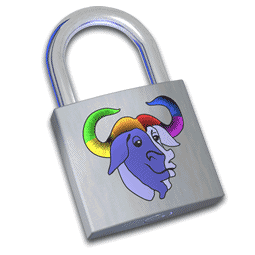
\includegraphics{images/gpg-logo.png}
%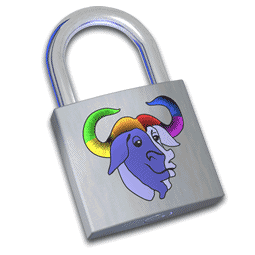
\includegraphics[scale=1]{images/gpg-logo.png}
\thispagestyle{empty}

%%\LARGE

%%\tableofcontents

\section{What is GPG?}

\textbf{GPG}, or GNU Privacy Guard is, in a nutshell, \textit{a free and easy way to send and receive emails completely securely}. The way most emails are currently sent is completely insecure, and is directly analogous to sending all of your mail on a postcard, available for any postman or eavesdropper along the way to read: we don't think this is good enough, and want to encourage more people to think and care about their privacy online.

\textbf{GPG} allows you to send \textbf{completely secure} emails to anyone else with an email address and a key: no special email provider is needed.

\section{How does it work?}
To make sure that only the intended recipient can read the email you've sent them, you need to encrypt the message. This means that to anyone without the right password (or `key') the message will look like random gibberish. \\As you may or may not have ever met the person you want to email, you probably won't have a way of agreeing a password without knowing for certain that no-one can intercept it (meaning they could read your messages too). Instead, as an analogy, you create an \textit{electronic padlock and key}, or \textbf{Public / Private Key Pair}. The Public Key is the padlock, and the Private Key is the key you use to unlock it. You mustn't send anyone a copy of the private key over the internet as someone could copy it, but instead you can send out an unlocked padlock (the public key) to anyone who wants to send you an email; this way they can `lock' (encrypt) the message with the padlock, but no-one, not even the sender can `unlock' (decrypt) it -- only you, the person with the private key can do that.\\ So that anyone can send you an email securely, you distribute your `open padlock' (Public Key) freely using a Key Server, such as \href{http://pgp.mit.edu}{http://pgp.mit.edu}. Anyone can type in your name or email address and find your public key this way, but don't worry, there's no way anyone can work backwards from the Public Key to work out anything about your Private Key.

\section{Setup and usage guide, Linux edition}
\textit{(If you are using Windows or Linux please go to CompSoc's GPG website, \href{http://gpg.compsoc.dur.ac.uk}{http://gpg.compsoc.dur.ac.uk}. Also go to the website for full screenshots of this walkthrough.)} \\
Please don't be put off by the 10 steps to this guide -- most of them are completely obvious when in GPGTools.
\begin{compactenum}[1.]%itemize}
    \item Going to show mostly command line stuff but with some Thunderbird.
\end{compactenum}%itemize}

\section{Key Management}

\subsection{Revocation}
You may have noticed the option of the `Expiration date' when you created your Key Pair - this is important.

Make sure you have a backup of your Public/Private Key Pair somewhere safe. But you already take full backups regularly anyway, don't you? :-)

Somewhere mention about saving drafts locally, not on the server?
















\loggingall
\end{document}
\endinput
%%
%% End of file `leaflet-manual.tex'.
